\documentclass[1p]{elsarticle_modified}
%\bibliographystyle{elsarticle-num}

%\usepackage[colorlinks]{hyperref}
%\usepackage{abbrmath_seonhwa} %\Abb, \Ascr, \Acal ,\Abf, \Afrak
\usepackage{amsfonts}
\usepackage{amssymb}
\usepackage{amsmath}
\usepackage{amsthm}
\usepackage{scalefnt}
\usepackage{amsbsy}
\usepackage{kotex}
\usepackage{caption}
\usepackage{subfig}
\usepackage{color}
\usepackage{graphicx}
\usepackage{xcolor} %% white, black, red, green, blue, cyan, magenta, yellow
\usepackage{float}
\usepackage{setspace}
\usepackage{hyperref}

\usepackage{tikz}
\usetikzlibrary{arrows}

\usepackage{multirow}
\usepackage{array} % fixed length table
\usepackage{hhline}

%%%%%%%%%%%%%%%%%%%%%
\makeatletter
\renewcommand*\env@matrix[1][\arraystretch]{%
	\edef\arraystretch{#1}%
	\hskip -\arraycolsep
	\let\@ifnextchar\new@ifnextchar
	\array{*\c@MaxMatrixCols c}}
\makeatother %https://tex.stackexchange.com/questions/14071/how-can-i-increase-the-line-spacing-in-a-matrix
%%%%%%%%%%%%%%%

\usepackage[normalem]{ulem}

\newcommand{\msout}[1]{\ifmmode\text{\sout{\ensuremath{#1}}}\else\sout{#1}\fi}
%SOURCE: \msout is \stkout macro in https://tex.stackexchange.com/questions/20609/strikeout-in-math-mode

\newcommand{\cancel}[1]{
	\ifmmode
	{\color{red}\msout{#1}}
	\else
	{\color{red}\sout{#1}}
	\fi
}

\newcommand{\add}[1]{
	{\color{blue}\uwave{#1}}
}

\newcommand{\replace}[2]{
	\ifmmode
	{\color{red}\msout{#1}}{\color{blue}\uwave{#2}}
	\else
	{\color{red}\sout{#1}}{\color{blue}\uwave{#2}}
	\fi
}

\newcommand{\Sol}{\mathcal{S}} %segment
\newcommand{\D}{D} %diagram
\newcommand{\A}{\mathcal{A}} %arc


%%%%%%%%%%%%%%%%%%%%%%%%%%%%%5 test

\def\sl{\operatorname{\textup{SL}}(2,\Cbb)}
\def\psl{\operatorname{\textup{PSL}}(2,\Cbb)}
\def\quan{\mkern 1mu \triangleright \mkern 1mu}

\theoremstyle{definition}
\newtheorem{thm}{Theorem}[section]
\newtheorem{prop}[thm]{Proposition}
\newtheorem{lem}[thm]{Lemma}
\newtheorem{ques}[thm]{Question}
\newtheorem{cor}[thm]{Corollary}
\newtheorem{defn}[thm]{Definition}
\newtheorem{exam}[thm]{Example}
\newtheorem{rmk}[thm]{Remark}
\newtheorem{alg}[thm]{Algorithm}

\newcommand{\I}{\sqrt{-1}}
\begin{document}

%\begin{frontmatter}
%
%\title{Boundary parabolic representations of knots up to 8 crossings}
%
%%% Group authors per affiliation:
%\author{Yunhi Cho} 
%\address{Department of Mathematics, University of Seoul, Seoul, Korea}
%\ead{yhcho@uos.ac.kr}
%
%
%\author{Seonhwa Kim} %\fnref{s_kim}}
%\address{Center for Geometry and Physics, Institute for Basic Science, Pohang, 37673, Korea}
%\ead{ryeona17@ibs.re.kr}
%
%\author{Hyuk Kim}
%\address{Department of Mathematical Sciences, Seoul National University, Seoul 08826, Korea}
%\ead{hyukkim@snu.ac.kr}
%
%\author{Seokbeom Yoon}
%\address{Department of Mathematical Sciences, Seoul National University, Seoul, 08826,  Korea}
%\ead{sbyoon15@snu.ac.kr}
%
%\begin{abstract}
%We find all boundary parabolic representation of knots up to 8 crossings.
%
%\end{abstract}
%\begin{keyword}
%    \MSC[2010] 57M25 
%\end{keyword}
%
%\end{frontmatter}

%\linenumbers
%\tableofcontents
%
\newcommand\colored[1]{\textcolor{white}{\rule[-0.35ex]{0.8em}{1.4ex}}\kern-0.8em\color{red} #1}%
%\newcommand\colored[1]{\textcolor{white}{ #1}\kern-2.17ex	\textcolor{white}{ #1}\kern-1.81ex	\textcolor{white}{ #1}\kern-2.15ex\color{red}#1	}

{\Large $\underline{12n_{0449}~(K12n_{0449})}$}

\setlength{\tabcolsep}{10pt}
\renewcommand{\arraystretch}{1.6}
\vspace{1cm}\begin{tabular}{m{100pt}>{\centering\arraybackslash}m{274pt}}
\multirow{5}{120pt}{
	\centering
	\includegraphics[width=112pt]{../../../GIT/diagram.site/Diagrams/png/2538_12n_0449.png}\\
\ \ \ A knot diagram\footnotemark}&
\allowdisplaybreaks
\textbf{Linearized knot diagam} \\
\cline{2-2}
 &
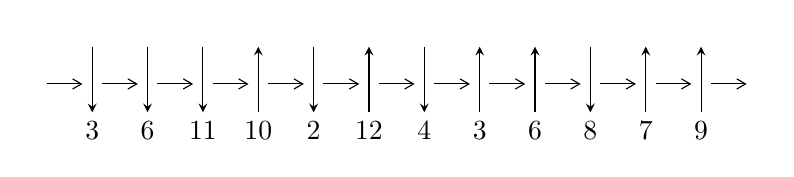
\begin{tikzpicture}[x=20pt, y=17pt]
	% nodes
	\node (C0) at (0, 0) {};
	\node (C1) at (1, 0) {};
	\node (C1U) at (1, +1) {};
	\node (C1D) at (1, -1) {3};

	\node (C2) at (2, 0) {};
	\node (C2U) at (2, +1) {};
	\node (C2D) at (2, -1) {6};

	\node (C3) at (3, 0) {};
	\node (C3U) at (3, +1) {};
	\node (C3D) at (3, -1) {11};

	\node (C4) at (4, 0) {};
	\node (C4U) at (4, +1) {};
	\node (C4D) at (4, -1) {10};

	\node (C5) at (5, 0) {};
	\node (C5U) at (5, +1) {};
	\node (C5D) at (5, -1) {2};

	\node (C6) at (6, 0) {};
	\node (C6U) at (6, +1) {};
	\node (C6D) at (6, -1) {12};

	\node (C7) at (7, 0) {};
	\node (C7U) at (7, +1) {};
	\node (C7D) at (7, -1) {4};

	\node (C8) at (8, 0) {};
	\node (C8U) at (8, +1) {};
	\node (C8D) at (8, -1) {3};

	\node (C9) at (9, 0) {};
	\node (C9U) at (9, +1) {};
	\node (C9D) at (9, -1) {6};

	\node (C10) at (10, 0) {};
	\node (C10U) at (10, +1) {};
	\node (C10D) at (10, -1) {8};

	\node (C11) at (11, 0) {};
	\node (C11U) at (11, +1) {};
	\node (C11D) at (11, -1) {7};

	\node (C12) at (12, 0) {};
	\node (C12U) at (12, +1) {};
	\node (C12D) at (12, -1) {9};
	\node (C13) at (13, 0) {};

	% arrows
	\draw[->,>={angle 60}]
	(C0) edge (C1) (C1) edge (C2) (C2) edge (C3) (C3) edge (C4) (C4) edge (C5) (C5) edge (C6) (C6) edge (C7) (C7) edge (C8) (C8) edge (C9) (C9) edge (C10) (C10) edge (C11) (C11) edge (C12) (C12) edge (C13) ;	\draw[->,>=stealth]
	(C1U) edge (C1D) (C2U) edge (C2D) (C3U) edge (C3D) (C4D) edge (C4U) (C5U) edge (C5D) (C6D) edge (C6U) (C7U) edge (C7D) (C8D) edge (C8U) (C9D) edge (C9U) (C10U) edge (C10D) (C11D) edge (C11U) (C12D) edge (C12U) ;
	\end{tikzpicture} \\
\hhline{~~} \\& 
\textbf{Solving Sequence} \\ \cline{2-2} 
 &
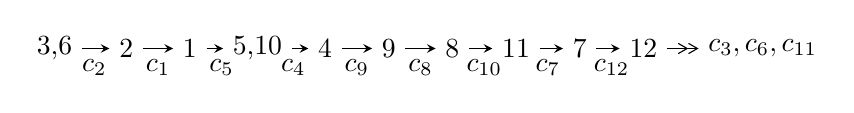
\begin{tikzpicture}[x=23pt, y=7pt]
	% node
	\node (A0) at (-1/8, 0) {3,6};
	\node (A1) at (1, 0) {2};
	\node (A2) at (2, 0) {1};
	\node (A3) at (49/16, 0) {5,10};
	\node (A4) at (33/8, 0) {4};
	\node (A5) at (41/8, 0) {9};
	\node (A6) at (49/8, 0) {8};
	\node (A7) at (57/8, 0) {11};
	\node (A8) at (65/8, 0) {7};
	\node (A9) at (73/8, 0) {12};
	\node (C1) at (1/2, -1) {$c_{2}$};
	\node (C2) at (3/2, -1) {$c_{1}$};
	\node (C3) at (5/2, -1) {$c_{5}$};
	\node (C4) at (29/8, -1) {$c_{4}$};
	\node (C5) at (37/8, -1) {$c_{9}$};
	\node (C6) at (45/8, -1) {$c_{8}$};
	\node (C7) at (53/8, -1) {$c_{10}$};
	\node (C8) at (61/8, -1) {$c_{7}$};
	\node (C9) at (69/8, -1) {$c_{12}$};
	\node (A10) at (11, 0) {$c_{3},c_{6},c_{11}$};

	% edge
	\draw[->,>=stealth]	
	(A0) edge (A1) (A1) edge (A2) (A2) edge (A3) (A3) edge (A4) (A4) edge (A5) (A5) edge (A6) (A6) edge (A7) (A7) edge (A8) (A8) edge (A9) ;
	\draw[->>,>={angle 60}]	
	(A9) edge (A10);
\end{tikzpicture} \\ 

\end{tabular} \\

\footnotetext{
The image of knot diagram is generated by the software ``\textbf{Draw programme}" developed by Andrew Bartholomew(\url{http://www.layer8.co.uk/maths/draw/index.htm\#Running-draw}), where we modified some parts for our purpose(\url{https://github.com/CATsTAILs/LinksPainter}).
}\phantom \\ \newline 
\centering \textbf{Ideals for irreducible components\footnotemark of $X_{\text{par}}$} 
 
\begin{align*}
I^u_{1}&=\langle 
-4292389719 u^{17}+51152895286 u^{16}+\cdots+4997872592 b-142666014976,\\
\phantom{I^u_{1}}&\phantom{= \langle  }635549962 u^{17}-7071211853 u^{16}+\cdots+4997872592 a+18555030320,\\
\phantom{I^u_{1}}&\phantom{= \langle  }u^{18}-14 u^{17}+\cdots-32 u-64\rangle \\
I^u_{2}&=\langle 
2861 u^{12}+19240 u^{11}+\cdots+3447 b-26153,\;-10868 u^{12}-66331 u^{11}+\cdots+17235 a+57767,\\
\phantom{I^u_{2}}&\phantom{= \langle  }u^{13}+7 u^{12}+18 u^{11}+18 u^{10}-5 u^9-30 u^8-29 u^7-5 u^6+22 u^5+26 u^4- u^3-25 u^2-19 u-5\rangle \\
I^u_{3}&=\langle 
-48036 a^5 u^2-192549 a^4 u^2+\cdots-3719319 a-1942337,\;a^5 u^2-3 a^4 u^2+\cdots+13 a+8,\;u^3+2 u^2+1\rangle \\
I^u_{4}&=\langle 
b^2+b a+a^2,\;a^3+a^2-1,\;u-1\rangle \\
\\
\end{align*}
\raggedright * 4 irreducible components of $\dim_{\mathbb{C}}=0$, with total 55 representations.\\
\footnotetext{All coefficients of polynomials are rational numbers. But the coefficients are sometimes approximated in decimal forms when there is not enough margin.}
\newpage
\renewcommand{\arraystretch}{1}
\centering \section*{I. $I^u_{1}= \langle -4.29\times10^{9} u^{17}+5.12\times10^{10} u^{16}+\cdots+5.00\times10^{9} b-1.43\times10^{11},\;6.36\times10^{8} u^{17}-7.07\times10^{9} u^{16}+\cdots+5.00\times10^{9} a+1.86\times10^{10},\;u^{18}-14 u^{17}+\cdots-32 u-64 \rangle$}
\flushleft \textbf{(i) Arc colorings}\\
\begin{tabular}{m{7pt} m{180pt} m{7pt} m{180pt} }
\flushright $a_{3}=$&$\begin{pmatrix}1\\0\end{pmatrix}$ \\
\flushright $a_{6}=$&$\begin{pmatrix}0\\u\end{pmatrix}$ \\
\flushright $a_{2}=$&$\begin{pmatrix}1\\- u^2\end{pmatrix}$ \\
\flushright $a_{1}=$&$\begin{pmatrix}- u^2+1\\- u^2\end{pmatrix}$ \\
\flushright $a_{5}=$&$\begin{pmatrix}u\\- u^3+u\end{pmatrix}$ \\
\flushright $a_{10}=$&$\begin{pmatrix}-0.127164 u^{17}+1.41484 u^{16}+\cdots+2.40021 u-3.71259\\0.858843 u^{17}-10.2349 u^{16}+\cdots+31.2801 u+28.5453\end{pmatrix}$ \\
\flushright $a_{4}=$&$\begin{pmatrix}-0.0537381 u^{17}+0.686664 u^{16}+\cdots-3.43651 u-1.95932\\0.0261593 u^{17}-0.244759 u^{16}+\cdots+4.59772 u+1.60130\end{pmatrix}$ \\
\flushright $a_{9}=$&$\begin{pmatrix}-0.127164 u^{17}+1.41484 u^{16}+\cdots+2.40021 u-3.71259\\-0.0465960 u^{17}+0.240296 u^{16}+\cdots+11.4471 u+5.15636\end{pmatrix}$ \\
\flushright $a_{8}=$&$\begin{pmatrix}-0.0805681 u^{17}+1.17455 u^{16}+\cdots-9.04691 u-8.86894\\-0.0465960 u^{17}+0.240296 u^{16}+\cdots+11.4471 u+5.15636\end{pmatrix}$ \\
\flushright $a_{11}=$&$\begin{pmatrix}0.161781 u^{17}-1.96128 u^{16}+\cdots+9.04249 u+3.48865\\0.189746 u^{17}-2.43818 u^{16}+\cdots+14.8327 u+10.0529\end{pmatrix}$ \\
\flushright $a_{7}=$&$\begin{pmatrix}0.119990 u^{17}-1.53654 u^{16}+\cdots+8.62391 u+4.68769\\0.458477 u^{17}-5.52095 u^{16}+\cdots+15.8725 u+14.8725\end{pmatrix}$ \\
\flushright $a_{12}=$&$\begin{pmatrix}0.0119305 u^{17}-0.112150 u^{16}+\cdots-0.757572 u+2.47991\\0.0656686 u^{17}-0.798814 u^{16}+\cdots+3.67894 u+3.43924\end{pmatrix}$\\&\end{tabular}
\flushleft \textbf{(ii) Obstruction class $= -1$}\\~\\
\flushleft \textbf{(iii) Cusp Shapes $= \frac{336395251}{1249468148} u^{17}-\frac{1919281435}{624734074} u^{16}+\cdots-\frac{4336282305}{312367037} u+\frac{1452677222}{312367037}$}\\~\\
\newpage\renewcommand{\arraystretch}{1}
\flushleft \textbf{(iv) u-Polynomials at the component}\newline \\
\begin{tabular}{m{50pt}|m{274pt}}
Crossings & \hspace{64pt}u-Polynomials at each crossing \\
\hline $$\begin{aligned}c_{1}\end{aligned}$$&$\begin{aligned}
&u^{18}+44 u^{17}+\cdots+58880 u+4096
\end{aligned}$\\
\hline $$\begin{aligned}c_{2},c_{5}\end{aligned}$$&$\begin{aligned}
&u^{18}+14 u^{17}+\cdots+32 u-64
\end{aligned}$\\
\hline $$\begin{aligned}c_{3},c_{7}\end{aligned}$$&$\begin{aligned}
&u^{18}+u^{17}+\cdots+u+1
\end{aligned}$\\
\hline $$\begin{aligned}c_{4},c_{8}\end{aligned}$$&$\begin{aligned}
&u^{18}+15 u^{16}+\cdots-2 u-1
\end{aligned}$\\
\hline $$\begin{aligned}c_{6},c_{11}\end{aligned}$$&$\begin{aligned}
&u^{18}-8 u^{17}+\cdots+66 u^2-4
\end{aligned}$\\
\hline $$\begin{aligned}c_{9},c_{12}\end{aligned}$$&$\begin{aligned}
&u^{18}+u^{17}+\cdots-29 u-1
\end{aligned}$\\
\hline $$\begin{aligned}c_{10}\end{aligned}$$&$\begin{aligned}
&u^{18}-17 u^{17}+\cdots-112 u+8
\end{aligned}$\\
\hline
\end{tabular}\\~\\
\newpage\renewcommand{\arraystretch}{1}
\flushleft \textbf{(v) Riley Polynomials at the component}\newline \\
\begin{tabular}{m{50pt}|m{274pt}}
Crossings & \hspace{64pt}Riley Polynomials at each crossing \\
\hline $$\begin{aligned}c_{1}\end{aligned}$$&$\begin{aligned}
&y^{18}-180 y^{17}+\cdots-1103757312 y+16777216
\end{aligned}$\\
\hline $$\begin{aligned}c_{2},c_{5}\end{aligned}$$&$\begin{aligned}
&y^{18}-44 y^{17}+\cdots-58880 y+4096
\end{aligned}$\\
\hline $$\begin{aligned}c_{3},c_{7}\end{aligned}$$&$\begin{aligned}
&y^{18}-9 y^{17}+\cdots+3 y+1
\end{aligned}$\\
\hline $$\begin{aligned}c_{4},c_{8}\end{aligned}$$&$\begin{aligned}
&y^{18}+30 y^{17}+\cdots-20 y+1
\end{aligned}$\\
\hline $$\begin{aligned}c_{6},c_{11}\end{aligned}$$&$\begin{aligned}
&y^{18}+12 y^{17}+\cdots-528 y+16
\end{aligned}$\\
\hline $$\begin{aligned}c_{9},c_{12}\end{aligned}$$&$\begin{aligned}
&y^{18}+43 y^{17}+\cdots-425 y+1
\end{aligned}$\\
\hline $$\begin{aligned}c_{10}\end{aligned}$$&$\begin{aligned}
&y^{18}-11 y^{17}+\cdots-1312 y+64
\end{aligned}$\\
\hline
\end{tabular}\\~\\
\newpage\flushleft \textbf{(vi) Complex Volumes and Cusp Shapes}
$$\begin{array}{c|c|c}  
\text{Solutions to }I^u_{1}& \I (\text{vol} + \sqrt{-1}CS) & \text{Cusp shape}\\
 \hline 
\begin{aligned}
u &= \phantom{-}0.899219\phantom{ +0.000000I} \\
a &= -0.0543767\phantom{ +0.000000I} \\
b &= \phantom{-}0.529143\phantom{ +0.000000I}\end{aligned}
 & -1.46517\phantom{ +0.000000I} & -7.81630\phantom{ +0.000000I} \\ \hline\begin{aligned}
u &= \phantom{-}1.054770 + 0.455060 I \\
a &= -0.286687 + 0.255744 I \\
b &= \phantom{-}0.697632 + 0.987067 I\end{aligned}
 & -2.44657 - 1.20776 I & -2.90617 + 2.14647 I \\ \hline\begin{aligned}
u &= \phantom{-}1.054770 - 0.455060 I \\
a &= -0.286687 - 0.255744 I \\
b &= \phantom{-}0.697632 - 0.987067 I\end{aligned}
 & -2.44657 + 1.20776 I & -2.90617 - 2.14647 I \\ \hline\begin{aligned}
u &= \phantom{-}1.182210 + 0.365563 I \\
a &= -0.196661 - 0.172033 I \\
b &= -0.688510 + 0.458421 I\end{aligned}
 & -4.86247 - 0.74221 I & -4.48012 - 1.53917 I \\ \hline\begin{aligned}
u &= \phantom{-}1.182210 - 0.365563 I \\
a &= -0.196661 + 0.172033 I \\
b &= -0.688510 - 0.458421 I\end{aligned}
 & -4.86247 + 0.74221 I & -4.48012 + 1.53917 I \\ \hline\begin{aligned}
u &= \phantom{-}0.011252 + 0.650614 I \\
a &= \phantom{-}0.249333 + 0.938849 I \\
b &= \phantom{-}0.628633 + 0.554074 I\end{aligned}
 & -1.41190 - 2.84945 I & \phantom{-}2.25914 + 3.12009 I \\ \hline\begin{aligned}
u &= \phantom{-}0.011252 - 0.650614 I \\
a &= \phantom{-}0.249333 - 0.938849 I \\
b &= \phantom{-}0.628633 - 0.554074 I\end{aligned}
 & -1.41190 + 2.84945 I & \phantom{-}2.25914 - 3.12009 I \\ \hline\begin{aligned}
u &= -1.56372\phantom{ +0.000000I} \\
a &= -1.20023\phantom{ +0.000000I} \\
b &= \phantom{-}2.20274\phantom{ +0.000000I}\end{aligned}
 & -1.13784\phantom{ +0.000000I} & -8.76730\phantom{ +0.000000I} \\ \hline\begin{aligned}
u &= -1.57964 + 0.17770 I \\
a &= \phantom{-}1.028070 + 0.171267 I \\
b &= -1.99303 + 0.23309 I\end{aligned}
 & -5.95294 + 6.24667 I & -5.65069 - 4.46750 I \\ \hline\begin{aligned}
u &= -1.57964 - 0.17770 I \\
a &= \phantom{-}1.028070 - 0.171267 I \\
b &= -1.99303 - 0.23309 I\end{aligned}
 & -5.95294 - 6.24667 I & -5.65069 + 4.46750 I\\
 \hline 
 \end{array}$$\newpage$$\begin{array}{c|c|c}  
\text{Solutions to }I^u_{1}& \I (\text{vol} + \sqrt{-1}CS) & \text{Cusp shape}\\
 \hline 
\begin{aligned}
u &= -0.337307 + 0.100488 I \\
a &= -1.45027 - 1.37394 I \\
b &= -0.205154 - 0.227150 I\end{aligned}
 & \phantom{-}1.118560 + 0.696320 I & \phantom{-}7.37877 - 3.46588 I \\ \hline\begin{aligned}
u &= -0.337307 - 0.100488 I \\
a &= -1.45027 + 1.37394 I \\
b &= -0.205154 + 0.227150 I\end{aligned}
 & \phantom{-}1.118560 - 0.696320 I & \phantom{-}7.37877 + 3.46588 I \\ \hline\begin{aligned}
u &= \phantom{-}2.31673 + 0.16616 I \\
a &= \phantom{-}0.176104 - 1.366420 I \\
b &= -1.81352 + 4.75613 I\end{aligned}
 & \phantom{-}17.0902 - 12.5383 I & -5.56236 + 5.19794 I \\ \hline\begin{aligned}
u &= \phantom{-}2.31673 - 0.16616 I \\
a &= \phantom{-}0.176104 + 1.366420 I \\
b &= -1.81352 - 4.75613 I\end{aligned}
 & \phantom{-}17.0902 + 12.5383 I & -5.56236 - 5.19794 I \\ \hline\begin{aligned}
u &= \phantom{-}2.30666 + 0.43513 I \\
a &= \phantom{-}0.124162 - 1.296380 I \\
b &= -3.32718 + 4.18498 I\end{aligned}
 & \phantom{-}18.8942 + 0.4671 I & -7.70038 + 0.38231 I \\ \hline\begin{aligned}
u &= \phantom{-}2.30666 - 0.43513 I \\
a &= \phantom{-}0.124162 + 1.296380 I \\
b &= -3.32718 - 4.18498 I\end{aligned}
 & \phantom{-}18.8942 - 0.4671 I & -7.70038 - 0.38231 I \\ \hline\begin{aligned}
u &= \phantom{-}2.37757 + 0.25374 I \\
a &= -0.141746 + 1.335690 I \\
b &= \phantom{-}2.33519 - 5.00160 I\end{aligned}
 & -17.0153 - 6.5912 I & -3.54637 + 4.05505 I \\ \hline\begin{aligned}
u &= \phantom{-}2.37757 - 0.25374 I \\
a &= -0.141746 - 1.335690 I \\
b &= \phantom{-}2.33519 + 5.00160 I\end{aligned}
 & -17.0153 + 6.5912 I & -3.54637 - 4.05505 I\\
 \hline 
 \end{array}$$\newpage\newpage\renewcommand{\arraystretch}{1}
\centering \section*{II. $I^u_{2}= \langle 2861 u^{12}+19240 u^{11}+\cdots+3447 b-26153,\;-10868 u^{12}-66331 u^{11}+\cdots+17235 a+57767,\;u^{13}+7 u^{12}+\cdots-19 u-5 \rangle$}
\flushleft \textbf{(i) Arc colorings}\\
\begin{tabular}{m{7pt} m{180pt} m{7pt} m{180pt} }
\flushright $a_{3}=$&$\begin{pmatrix}1\\0\end{pmatrix}$ \\
\flushright $a_{6}=$&$\begin{pmatrix}0\\u\end{pmatrix}$ \\
\flushright $a_{2}=$&$\begin{pmatrix}1\\- u^2\end{pmatrix}$ \\
\flushright $a_{1}=$&$\begin{pmatrix}- u^2+1\\- u^2\end{pmatrix}$ \\
\flushright $a_{5}=$&$\begin{pmatrix}u\\- u^3+u\end{pmatrix}$ \\
\flushright $a_{10}=$&$\begin{pmatrix}0.630577 u^{12}+3.84862 u^{11}+\cdots-10.2507 u-3.35173\\-0.829997 u^{12}-5.58167 u^{11}+\cdots+17.5666 u+7.58718\end{pmatrix}$ \\
\flushright $a_{4}=$&$\begin{pmatrix}-0.00765883 u^{12}-0.137163 u^{11}+\cdots+1.89643 u-0.681288\\0.0478677 u^{12}+0.190601 u^{11}+\cdots-1.76936 u-0.908616\end{pmatrix}$ \\
\flushright $a_{9}=$&$\begin{pmatrix}0.630577 u^{12}+3.84862 u^{11}+\cdots-10.2507 u-3.35173\\-0.321439 u^{12}-2.49405 u^{11}+\cdots+9.97650 u+4.76008\end{pmatrix}$ \\
\flushright $a_{8}=$&$\begin{pmatrix}0.952016 u^{12}+6.34267 u^{11}+\cdots-20.2272 u-8.11181\\-0.321439 u^{12}-2.49405 u^{11}+\cdots+9.97650 u+4.76008\end{pmatrix}$ \\
\flushright $a_{11}=$&$\begin{pmatrix}0.265390 u^{12}+1.06603 u^{11}+\cdots+2.70496 u+4.37534\\-1.05628 u^{12}-6.69481 u^{11}+\cdots+18.3551 u+5.76124\end{pmatrix}$ \\
\flushright $a_{7}=$&$\begin{pmatrix}-0.526429 u^{12}-2.96321 u^{11}+\cdots+4.12620 u-0.318132\\-0.0272701 u^{12}+0.319698 u^{11}+\cdots-4.18190 u-1.79954\end{pmatrix}$ \\
\flushright $a_{12}=$&$\begin{pmatrix}0.0912097 u^{12}+0.512272 u^{11}+\cdots-0.0696258 u+1.71958\\0.0835509 u^{12}+0.375109 u^{11}+\cdots+0.826806 u+0.0382942\end{pmatrix}$\\&\end{tabular}
\flushleft \textbf{(ii) Obstruction class $= 1$}\\~\\
\flushleft \textbf{(iii) Cusp Shapes $= \frac{9460}{3447} u^{12}+\frac{61031}{3447} u^{11}+\cdots-\frac{23618}{383} u-\frac{94159}{3447}$}\\~\\
\newpage\renewcommand{\arraystretch}{1}
\flushleft \textbf{(iv) u-Polynomials at the component}\newline \\
\begin{tabular}{m{50pt}|m{274pt}}
Crossings & \hspace{64pt}u-Polynomials at each crossing \\
\hline $$\begin{aligned}c_{1}\end{aligned}$$&$\begin{aligned}
&u^{13}-13 u^{12}+\cdots+111 u-25
\end{aligned}$\\
\hline $$\begin{aligned}c_{2}\end{aligned}$$&$\begin{aligned}
&u^{13}+7 u^{12}+\cdots-19 u-5
\end{aligned}$\\
\hline $$\begin{aligned}c_{3},c_{7}\end{aligned}$$&$\begin{aligned}
&u^{13}- u^{12}+\cdots+2 u+1
\end{aligned}$\\
\hline $$\begin{aligned}c_{4},c_{8}\end{aligned}$$&$\begin{aligned}
&u^{13}+9 u^{11}+\cdots+u+1
\end{aligned}$\\
\hline $$\begin{aligned}c_{5}\end{aligned}$$&$\begin{aligned}
&u^{13}-7 u^{12}+\cdots-19 u+5
\end{aligned}$\\
\hline $$\begin{aligned}c_{6}\end{aligned}$$&$\begin{aligned}
&u^{13}-3 u^{12}+\cdots-10 u+4
\end{aligned}$\\
\hline $$\begin{aligned}c_{9},c_{12}\end{aligned}$$&$\begin{aligned}
&u^{13}- u^{12}+\cdots+2 u-1
\end{aligned}$\\
\hline $$\begin{aligned}c_{10}\end{aligned}$$&$\begin{aligned}
&u^{13}+8 u^{12}+\cdots-99 u-27
\end{aligned}$\\
\hline $$\begin{aligned}c_{11}\end{aligned}$$&$\begin{aligned}
&u^{13}+3 u^{12}+\cdots-10 u-4
\end{aligned}$\\
\hline
\end{tabular}\\~\\
\newpage\renewcommand{\arraystretch}{1}
\flushleft \textbf{(v) Riley Polynomials at the component}\newline \\
\begin{tabular}{m{50pt}|m{274pt}}
Crossings & \hspace{64pt}Riley Polynomials at each crossing \\
\hline $$\begin{aligned}c_{1}\end{aligned}$$&$\begin{aligned}
&y^{13}-45 y^{12}+\cdots-4029 y-625
\end{aligned}$\\
\hline $$\begin{aligned}c_{2},c_{5}\end{aligned}$$&$\begin{aligned}
&y^{13}-13 y^{12}+\cdots+111 y-25
\end{aligned}$\\
\hline $$\begin{aligned}c_{3},c_{7}\end{aligned}$$&$\begin{aligned}
&y^{13}-5 y^{12}+\cdots+16 y-1
\end{aligned}$\\
\hline $$\begin{aligned}c_{4},c_{8}\end{aligned}$$&$\begin{aligned}
&y^{13}+18 y^{12}+\cdots-9 y-1
\end{aligned}$\\
\hline $$\begin{aligned}c_{6},c_{11}\end{aligned}$$&$\begin{aligned}
&y^{13}+9 y^{12}+\cdots-20 y-16
\end{aligned}$\\
\hline $$\begin{aligned}c_{9},c_{12}\end{aligned}$$&$\begin{aligned}
&y^{13}+15 y^{12}+\cdots+8 y^2-1
\end{aligned}$\\
\hline $$\begin{aligned}c_{10}\end{aligned}$$&$\begin{aligned}
&y^{13}-8 y^{12}+\cdots+3807 y-729
\end{aligned}$\\
\hline
\end{tabular}\\~\\
\newpage\flushleft \textbf{(vi) Complex Volumes and Cusp Shapes}
$$\begin{array}{c|c|c}  
\text{Solutions to }I^u_{2}& \I (\text{vol} + \sqrt{-1}CS) & \text{Cusp shape}\\
 \hline 
\begin{aligned}
u &= \phantom{-}0.856243 + 0.439666 I \\
a &= \phantom{-}0.053687 + 1.058490 I \\
b &= \phantom{-}0.666388 - 0.086808 I\end{aligned}
 & -5.33979 - 2.00841 I & -6.30003 + 4.09243 I \\ \hline\begin{aligned}
u &= \phantom{-}0.856243 - 0.439666 I \\
a &= \phantom{-}0.053687 - 1.058490 I \\
b &= \phantom{-}0.666388 + 0.086808 I\end{aligned}
 & -5.33979 + 2.00841 I & -6.30003 - 4.09243 I \\ \hline\begin{aligned}
u &= -0.056167 + 1.060590 I \\
a &= -0.794885 - 0.705726 I \\
b &= -0.85889 - 1.67983 I\end{aligned}
 & -3.27208 - 3.50308 I & -5.03802 + 3.23691 I \\ \hline\begin{aligned}
u &= -0.056167 - 1.060590 I \\
a &= -0.794885 + 0.705726 I \\
b &= -0.85889 + 1.67983 I\end{aligned}
 & -3.27208 + 3.50308 I & -5.03802 - 3.23691 I \\ \hline\begin{aligned}
u &= \phantom{-}1.10413\phantom{ +0.000000I} \\
a &= \phantom{-}0.938401\phantom{ +0.000000I} \\
b &= -0.651589\phantom{ +0.000000I}\end{aligned}
 & -0.224822\phantom{ +0.000000I} & \phantom{-}1.29960\phantom{ +0.000000I} \\ \hline\begin{aligned}
u &= -1.074570 + 0.503982 I \\
a &= -0.476495 - 0.014009 I \\
b &= -0.14184 - 1.44672 I\end{aligned}
 & -5.72718 + 8.88579 I & -3.64178 - 7.62615 I \\ \hline\begin{aligned}
u &= -1.074570 - 0.503982 I \\
a &= -0.476495 + 0.014009 I \\
b &= -0.14184 + 1.44672 I\end{aligned}
 & -5.72718 - 8.88579 I & -3.64178 + 7.62615 I \\ \hline\begin{aligned}
u &= -1.033670 + 0.730191 I \\
a &= \phantom{-}0.539770 + 0.500315 I \\
b &= -1.15414 + 1.81649 I\end{aligned}
 & -3.61034 + 0.42465 I & -7.93042 + 0.83468 I \\ \hline\begin{aligned}
u &= -1.033670 - 0.730191 I \\
a &= \phantom{-}0.539770 - 0.500315 I \\
b &= -1.15414 - 1.81649 I\end{aligned}
 & -3.61034 - 0.42465 I & -7.93042 - 0.83468 I \\ \hline\begin{aligned}
u &= -0.537801 + 0.322672 I \\
a &= \phantom{-}0.581072 - 0.696232 I \\
b &= \phantom{-}0.576934 + 1.237160 I\end{aligned}
 & -1.38260 + 4.11097 I & -0.96481 - 7.32347 I\\
 \hline 
 \end{array}$$\newpage$$\begin{array}{c|c|c}  
\text{Solutions to }I^u_{2}& \I (\text{vol} + \sqrt{-1}CS) & \text{Cusp shape}\\
 \hline 
\begin{aligned}
u &= -0.537801 - 0.322672 I \\
a &= \phantom{-}0.581072 + 0.696232 I \\
b &= \phantom{-}0.576934 - 1.237160 I\end{aligned}
 & -1.38260 - 4.11097 I & -0.96481 + 7.32347 I \\ \hline\begin{aligned}
u &= -2.20610 + 0.12523 I \\
a &= \phantom{-}0.027651 - 1.287690 I \\
b &= \phantom{-}0.73733 + 3.92048 I\end{aligned}
 & -18.3891 - 1.5099 I & -4.27475 + 0.24744 I \\ \hline\begin{aligned}
u &= -2.20610 - 0.12523 I \\
a &= \phantom{-}0.027651 + 1.287690 I \\
b &= \phantom{-}0.73733 - 3.92048 I\end{aligned}
 & -18.3891 + 1.5099 I & -4.27475 - 0.24744 I\\
 \hline 
 \end{array}$$\newpage\newpage\renewcommand{\arraystretch}{1}
\centering \section*{III. $I^u_{3}= \langle -4.80\times10^{4} a^{5} u^{2}-1.93\times10^{5} a^{4} u^{2}+\cdots-3.72\times10^{6} a-1.94\times10^{6},\;a^5 u^2-3 a^4 u^2+\cdots+13 a+8,\;u^3+2 u^2+1 \rangle$}
\flushleft \textbf{(i) Arc colorings}\\
\begin{tabular}{m{7pt} m{180pt} m{7pt} m{180pt} }
\flushright $a_{3}=$&$\begin{pmatrix}1\\0\end{pmatrix}$ \\
\flushright $a_{6}=$&$\begin{pmatrix}0\\u\end{pmatrix}$ \\
\flushright $a_{2}=$&$\begin{pmatrix}1\\- u^2\end{pmatrix}$ \\
\flushright $a_{1}=$&$\begin{pmatrix}- u^2+1\\- u^2\end{pmatrix}$ \\
\flushright $a_{5}=$&$\begin{pmatrix}u\\2 u^2+u+1\end{pmatrix}$ \\
\flushright $a_{10}=$&$\begin{pmatrix}a\\0.0107216 a^{5} u^{2}+0.0429770 a^{4} u^{2}+\cdots+0.830153 a+0.433530\end{pmatrix}$ \\
\flushright $a_{4}=$&$\begin{pmatrix}-0.0276588 a^{5} u^{2}+0.0409242 a^{4} u^{2}+\cdots-0.707287 a+0.0149656\\0.0276588 a^{5} u^{2}-0.0409242 a^{4} u^{2}+\cdots+0.707287 a+0.985034\end{pmatrix}$ \\
\flushright $a_{9}=$&$\begin{pmatrix}a\\0.0107216 a^{5} u^{2}+0.0429770 a^{4} u^{2}+\cdots+0.830153 a+0.433530\end{pmatrix}$ \\
\flushright $a_{8}=$&$\begin{pmatrix}-0.0107216 a^{5} u^{2}-0.0429770 a^{4} u^{2}+\cdots+0.169847 a-0.433530\\0.0107216 a^{5} u^{2}+0.0429770 a^{4} u^{2}+\cdots+0.830153 a+0.433530\end{pmatrix}$ \\
\flushright $a_{11}=$&$\begin{pmatrix}-0.114428 a^{5} u^{2}+0.0317676 a^{4} u^{2}+\cdots-0.244681 a+1.20229\\0.125150 a^{5} u^{2}+0.0112093 a^{4} u^{2}+\cdots+1.07483 a-0.768759\end{pmatrix}$ \\
\flushright $a_{7}=$&$\begin{pmatrix}-0.0212085 a^{5} u^{2}+0.145939 a^{4} u^{2}+\cdots-1.19184 a+0.989840\\0.379146 a^{5} u^{2}+0.374514 a^{4} u^{2}+\cdots+0.519904 a+0.992191\end{pmatrix}$ \\
\flushright $a_{12}=$&$\begin{pmatrix}-0.135637 a^{5} u^{2}+0.177707 a^{4} u^{2}+\cdots-1.43652 a+2.19213\\-0.164698 a^{5} u^{2}+0.0554376 a^{4} u^{2}+\cdots+0.353544 a-1.34279\end{pmatrix}$\\&\end{tabular}
\flushleft \textbf{(ii) Obstruction class $= -1$}\\~\\
\flushleft \textbf{(iii) Cusp Shapes $= -\frac{877944}{2240141} a^5 u^2-\frac{2031720}{2240141} a^4 u^2+\cdots+\frac{2110148}{2240141} a-\frac{15981979}{2240141}$}\\~\\
\newpage\renewcommand{\arraystretch}{1}
\flushleft \textbf{(iv) u-Polynomials at the component}\newline \\
\begin{tabular}{m{50pt}|m{274pt}}
Crossings & \hspace{64pt}u-Polynomials at each crossing \\
\hline $$\begin{aligned}c_{1}\end{aligned}$$&$\begin{aligned}
&(u^3+4 u^2-4 u+1)^6
\end{aligned}$\\
\hline $$\begin{aligned}c_{2},c_{5}\end{aligned}$$&$\begin{aligned}
&(u^3-2 u^2-1)^6
\end{aligned}$\\
\hline $$\begin{aligned}c_{3},c_{7}\end{aligned}$$&$\begin{aligned}
&u^{18}+2 u^{17}+\cdots-129 u^2+27
\end{aligned}$\\
\hline $$\begin{aligned}c_{4},c_{8}\end{aligned}$$&$\begin{aligned}
&u^{18}+20 u^{16}+\cdots+180 u+11
\end{aligned}$\\
\hline $$\begin{aligned}c_{6},c_{11}\end{aligned}$$&$\begin{aligned}
&(u^3+u^2+2 u+1)^6
\end{aligned}$\\
\hline $$\begin{aligned}c_{9},c_{12}\end{aligned}$$&$\begin{aligned}
&u^{18}-3 u^{17}+\cdots+4276 u+383
\end{aligned}$\\
\hline $$\begin{aligned}c_{10}\end{aligned}$$&$\begin{aligned}
&(u^3+u^2- u-2)^6
\end{aligned}$\\
\hline
\end{tabular}\\~\\
\newpage\renewcommand{\arraystretch}{1}
\flushleft \textbf{(v) Riley Polynomials at the component}\newline \\
\begin{tabular}{m{50pt}|m{274pt}}
Crossings & \hspace{64pt}Riley Polynomials at each crossing \\
\hline $$\begin{aligned}c_{1}\end{aligned}$$&$\begin{aligned}
&(y^3-24 y^2+8 y-1)^6
\end{aligned}$\\
\hline $$\begin{aligned}c_{2},c_{5}\end{aligned}$$&$\begin{aligned}
&(y^3-4 y^2-4 y-1)^6
\end{aligned}$\\
\hline $$\begin{aligned}c_{3},c_{7}\end{aligned}$$&$\begin{aligned}
&y^{18}-4 y^{17}+\cdots-6966 y+729
\end{aligned}$\\
\hline $$\begin{aligned}c_{4},c_{8}\end{aligned}$$&$\begin{aligned}
&y^{18}+40 y^{17}+\cdots-15834 y+121
\end{aligned}$\\
\hline $$\begin{aligned}c_{6},c_{11}\end{aligned}$$&$\begin{aligned}
&(y^3+3 y^2+2 y-1)^6
\end{aligned}$\\
\hline $$\begin{aligned}c_{9},c_{12}\end{aligned}$$&$\begin{aligned}
&y^{18}+49 y^{17}+\cdots-7285948 y+146689
\end{aligned}$\\
\hline $$\begin{aligned}c_{10}\end{aligned}$$&$\begin{aligned}
&(y^3-3 y^2+5 y-4)^6
\end{aligned}$\\
\hline
\end{tabular}\\~\\
\newpage\flushleft \textbf{(vi) Complex Volumes and Cusp Shapes}
$$\begin{array}{c|c|c}  
\text{Solutions to }I^u_{3}& \I (\text{vol} + \sqrt{-1}CS) & \text{Cusp shape}\\
 \hline 
\begin{aligned}
u &= \phantom{-}0.102785 + 0.665457 I \\
a &= -0.271547 + 1.307830 I \\
b &= -0.22345 + 1.73716 I\end{aligned}
 & -1.13951 - 2.56897 I & -0.10440 + 2.13317 I \\ \hline\begin{aligned}
u &= \phantom{-}0.102785 + 0.665457 I \\
a &= -1.48693 - 0.70223 I \\
b &= -0.624969 - 0.126877 I\end{aligned}
 & -1.13951 - 2.56897 I & -0.10440 + 2.13317 I \\ \hline\begin{aligned}
u &= \phantom{-}0.102785 + 0.665457 I \\
a &= \phantom{-}1.56533 + 0.54666 I \\
b &= -0.121877 + 0.223759 I\end{aligned}
 & -5.27710 - 5.39709 I & -6.63367 + 5.11262 I \\ \hline\begin{aligned}
u &= \phantom{-}0.102785 + 0.665457 I \\
a &= -0.029119 + 0.292106 I \\
b &= \phantom{-}0.310540 - 1.045640 I\end{aligned}
 & -5.27710 + 0.25915 I & -6.63367 - 0.84628 I \\ \hline\begin{aligned}
u &= \phantom{-}0.102785 + 0.665457 I \\
a &= \phantom{-}2.67067 + 0.73911 I \\
b &= \phantom{-}2.26454 + 0.01108 I\end{aligned}
 & -5.27710 + 0.25915 I & -6.63367 - 0.84628 I \\ \hline\begin{aligned}
u &= \phantom{-}0.102785 + 0.665457 I \\
a &= -0.11892 - 2.98573 I \\
b &= -0.48087 - 2.93264 I\end{aligned}
 & -5.27710 - 5.39709 I & -6.63367 + 5.11262 I \\ \hline\begin{aligned}
u &= \phantom{-}0.102785 - 0.665457 I \\
a &= -0.271547 - 1.307830 I \\
b &= -0.22345 - 1.73716 I\end{aligned}
 & -1.13951 + 2.56897 I & -0.10440 - 2.13317 I \\ \hline\begin{aligned}
u &= \phantom{-}0.102785 - 0.665457 I \\
a &= -1.48693 + 0.70223 I \\
b &= -0.624969 + 0.126877 I\end{aligned}
 & -1.13951 + 2.56897 I & -0.10440 - 2.13317 I \\ \hline\begin{aligned}
u &= \phantom{-}0.102785 - 0.665457 I \\
a &= \phantom{-}1.56533 - 0.54666 I \\
b &= -0.121877 - 0.223759 I\end{aligned}
 & -5.27710 + 5.39709 I & -6.63367 - 5.11262 I \\ \hline\begin{aligned}
u &= \phantom{-}0.102785 - 0.665457 I \\
a &= -0.029119 - 0.292106 I \\
b &= \phantom{-}0.310540 + 1.045640 I\end{aligned}
 & -5.27710 - 0.25915 I & -6.63367 + 0.84628 I\\
 \hline 
 \end{array}$$\newpage$$\begin{array}{c|c|c}  
\text{Solutions to }I^u_{3}& \I (\text{vol} + \sqrt{-1}CS) & \text{Cusp shape}\\
 \hline 
\begin{aligned}
u &= \phantom{-}0.102785 - 0.665457 I \\
a &= \phantom{-}2.67067 - 0.73911 I \\
b &= \phantom{-}2.26454 - 0.01108 I\end{aligned}
 & -5.27710 - 0.25915 I & -6.63367 + 0.84628 I \\ \hline\begin{aligned}
u &= \phantom{-}0.102785 - 0.665457 I \\
a &= -0.11892 + 2.98573 I \\
b &= -0.48087 + 2.93264 I\end{aligned}
 & -5.27710 + 5.39709 I & -6.63367 - 5.11262 I \\ \hline\begin{aligned}
u &= -2.20557\phantom{ +0.000000I} \\
a &= -0.132067 + 1.061970 I \\
b &= \phantom{-}0.73082 - 2.94300 I\end{aligned}
 & \phantom{-}19.5761 + 2.8281 I & -8.26193 - 2.97945 I \\ \hline\begin{aligned}
u &= -2.20557\phantom{ +0.000000I} \\
a &= -0.132067 - 1.061970 I \\
b &= \phantom{-}0.73082 + 2.94300 I\end{aligned}
 & \phantom{-}19.5761 - 2.8281 I & -8.26193 + 2.97945 I \\ \hline\begin{aligned}
u &= -2.20557\phantom{ +0.000000I} \\
a &= \phantom{-}0.248720 + 1.254260 I \\
b &= -1.03878 - 3.80675 I\end{aligned}
 & -15.7648\phantom{ +0.000000I} & -1.73266 + 0. I\phantom{ +0.000000I} \\ \hline\begin{aligned}
u &= -2.20557\phantom{ +0.000000I} \\
a &= \phantom{-}0.248720 - 1.254260 I \\
b &= -1.03878 + 3.80675 I\end{aligned}
 & -15.7648\phantom{ +0.000000I} & -1.73266 + 0. I\phantom{ +0.000000I} \\ \hline\begin{aligned}
u &= -2.20557\phantom{ +0.000000I} \\
a &= -0.44614 + 1.55281 I \\
b &= \phantom{-}1.68404 - 4.99299 I\end{aligned}
 & \phantom{-}19.5761 - 2.8281 I & -8.26193 + 2.97945 I \\ \hline\begin{aligned}
u &= -2.20557\phantom{ +0.000000I} \\
a &= -0.44614 - 1.55281 I \\
b &= \phantom{-}1.68404 + 4.99299 I\end{aligned}
 & \phantom{-}19.5761 + 2.8281 I & -8.26193 - 2.97945 I\\
 \hline 
 \end{array}$$\newpage\newpage\renewcommand{\arraystretch}{1}
\centering \section*{IV. $I^u_{4}= \langle b^2+b a+a^2,\;a^3+a^2-1,\;u-1 \rangle$}
\flushleft \textbf{(i) Arc colorings}\\
\begin{tabular}{m{7pt} m{180pt} m{7pt} m{180pt} }
\flushright $a_{3}=$&$\begin{pmatrix}1\\0\end{pmatrix}$ \\
\flushright $a_{6}=$&$\begin{pmatrix}0\\1\end{pmatrix}$ \\
\flushright $a_{2}=$&$\begin{pmatrix}1\\-1\end{pmatrix}$ \\
\flushright $a_{1}=$&$\begin{pmatrix}0\\-1\end{pmatrix}$ \\
\flushright $a_{5}=$&$\begin{pmatrix}1\\0\end{pmatrix}$ \\
\flushright $a_{10}=$&$\begin{pmatrix}a\\b\end{pmatrix}$ \\
\flushright $a_{4}=$&$\begin{pmatrix}b a+1\\- b a- a^2\end{pmatrix}$ \\
\flushright $a_{9}=$&$\begin{pmatrix}a\\b+a\end{pmatrix}$ \\
\flushright $a_{8}=$&$\begin{pmatrix}- b\\b+a\end{pmatrix}$ \\
\flushright $a_{11}=$&$\begin{pmatrix}a\\b\end{pmatrix}$ \\
\flushright $a_{7}=$&$\begin{pmatrix}a^2+a-1\\- a^2 b+b+a\end{pmatrix}$ \\
\flushright $a_{12}=$&$\begin{pmatrix}a^2\\b a+a^2-1\end{pmatrix}$\\&\end{tabular}
\flushleft \textbf{(ii) Obstruction class $= 1$}\\~\\
\flushleft \textbf{(iii) Cusp Shapes $= 4 a-3$}\\~\\
\newpage\renewcommand{\arraystretch}{1}
\flushleft \textbf{(iv) u-Polynomials at the component}\newline \\
\begin{tabular}{m{50pt}|m{274pt}}
Crossings & \hspace{64pt}u-Polynomials at each crossing \\
\hline $$\begin{aligned}c_{1},c_{2}\end{aligned}$$&$\begin{aligned}
&(u-1)^6
\end{aligned}$\\
\hline $$\begin{aligned}c_{3},c_{4},c_{7}\\c_{8}\end{aligned}$$&$\begin{aligned}
&u^6- u^5+u^4-2 u^3+u^2+1
\end{aligned}$\\
\hline $$\begin{aligned}c_{5}\end{aligned}$$&$\begin{aligned}
&(u+1)^6
\end{aligned}$\\
\hline $$\begin{aligned}c_{6}\end{aligned}$$&$\begin{aligned}
&(u^3+u^2+2 u+1)^2
\end{aligned}$\\
\hline $$\begin{aligned}c_{9},c_{12}\end{aligned}$$&$\begin{aligned}
&(u^3+u^2-1)^2
\end{aligned}$\\
\hline $$\begin{aligned}c_{10}\end{aligned}$$&$\begin{aligned}
&u^6
\end{aligned}$\\
\hline $$\begin{aligned}c_{11}\end{aligned}$$&$\begin{aligned}
&(u^3- u^2+2 u-1)^2
\end{aligned}$\\
\hline
\end{tabular}\\~\\
\newpage\renewcommand{\arraystretch}{1}
\flushleft \textbf{(v) Riley Polynomials at the component}\newline \\
\begin{tabular}{m{50pt}|m{274pt}}
Crossings & \hspace{64pt}Riley Polynomials at each crossing \\
\hline $$\begin{aligned}c_{1},c_{2},c_{5}\end{aligned}$$&$\begin{aligned}
&(y-1)^6
\end{aligned}$\\
\hline $$\begin{aligned}c_{3},c_{4},c_{7}\\c_{8}\end{aligned}$$&$\begin{aligned}
&y^6+y^5- y^4+3 y^2+2 y+1
\end{aligned}$\\
\hline $$\begin{aligned}c_{6},c_{11}\end{aligned}$$&$\begin{aligned}
&(y^3+3 y^2+2 y-1)^2
\end{aligned}$\\
\hline $$\begin{aligned}c_{9},c_{12}\end{aligned}$$&$\begin{aligned}
&(y^3- y^2+2 y-1)^2
\end{aligned}$\\
\hline $$\begin{aligned}c_{10}\end{aligned}$$&$\begin{aligned}
&y^6
\end{aligned}$\\
\hline
\end{tabular}\\~\\
\newpage\flushleft \textbf{(vi) Complex Volumes and Cusp Shapes}
$$\begin{array}{c|c|c}  
\text{Solutions to }I^u_{4}& \I (\text{vol} + \sqrt{-1}CS) & \text{Cusp shape}\\
 \hline 
\begin{aligned}
u &= \phantom{-}1.00000\phantom{ +0.000000I} \\
a &= -0.877439 + 0.744862 I \\
b &= \phantom{-}1.083790 + 0.387453 I\end{aligned}
 & -4.66906 - 2.82812 I & -6.50976 + 2.97945 I \\ \hline\begin{aligned}
u &= \phantom{-}1.00000\phantom{ +0.000000I} \\
a &= -0.877439 + 0.744862 I \\
b &= -0.206350 - 1.132320 I\end{aligned}
 & -4.66906 - 2.82812 I & -6.50976 + 2.97945 I \\ \hline\begin{aligned}
u &= \phantom{-}1.00000\phantom{ +0.000000I} \\
a &= -0.877439 - 0.744862 I \\
b &= \phantom{-}1.083790 - 0.387453 I\end{aligned}
 & -4.66906 + 2.82812 I & -6.50976 - 2.97945 I \\ \hline\begin{aligned}
u &= \phantom{-}1.00000\phantom{ +0.000000I} \\
a &= -0.877439 - 0.744862 I \\
b &= -0.206350 + 1.132320 I\end{aligned}
 & -4.66906 + 2.82812 I & -6.50976 - 2.97945 I \\ \hline\begin{aligned}
u &= \phantom{-}1.00000\phantom{ +0.000000I} \\
a &= \phantom{-}0.754878\phantom{ +0.000000I} \\
b &= -0.377439 + 0.653743 I\end{aligned}
 & -0.531480\phantom{ +0.000000I} & \phantom{-}0.0195110\phantom{ +0.000000I} \\ \hline\begin{aligned}
u &= \phantom{-}1.00000\phantom{ +0.000000I} \\
a &= \phantom{-}0.754878\phantom{ +0.000000I} \\
b &= -0.377439 - 0.653743 I\end{aligned}
 & -0.531480\phantom{ +0.000000I} & \phantom{-}0.0195110\phantom{ +0.000000I}\\
 \hline 
 \end{array}$$\newpage
\newpage\renewcommand{\arraystretch}{1}
\centering \section*{ V. u-Polynomials}
\begin{tabular}{m{50pt}|m{274pt}}
Crossings & \hspace{64pt}u-Polynomials at each crossing \\
\hline $$\begin{aligned}c_{1}\end{aligned}$$&$\begin{aligned}
&((u-1)^6)(u^3+4 u^2-4 u+1)^6(u^{13}-13 u^{12}+\cdots+111 u-25)\\
&\cdot(u^{18}+44 u^{17}+\cdots+58880 u+4096)
\end{aligned}$\\
\hline $$\begin{aligned}c_{2}\end{aligned}$$&$\begin{aligned}
&((u-1)^6)(u^3-2 u^2-1)^6(u^{13}+7 u^{12}+\cdots-19 u-5)\\
&\cdot(u^{18}+14 u^{17}+\cdots+32 u-64)
\end{aligned}$\\
\hline $$\begin{aligned}c_{3},c_{7}\end{aligned}$$&$\begin{aligned}
&(u^6- u^5+u^4-2 u^3+u^2+1)(u^{13}- u^{12}+\cdots+2 u+1)\\
&\cdot(u^{18}+u^{17}+\cdots+u+1)(u^{18}+2 u^{17}+\cdots-129 u^2+27)
\end{aligned}$\\
\hline $$\begin{aligned}c_{4},c_{8}\end{aligned}$$&$\begin{aligned}
&(u^6- u^5+u^4-2 u^3+u^2+1)(u^{13}+9 u^{11}+\cdots+u+1)\\
&\cdot(u^{18}+15 u^{16}+\cdots-2 u-1)(u^{18}+20 u^{16}+\cdots+180 u+11)
\end{aligned}$\\
\hline $$\begin{aligned}c_{5}\end{aligned}$$&$\begin{aligned}
&((u+1)^6)(u^3-2 u^2-1)^6(u^{13}-7 u^{12}+\cdots-19 u+5)\\
&\cdot(u^{18}+14 u^{17}+\cdots+32 u-64)
\end{aligned}$\\
\hline $$\begin{aligned}c_{6}\end{aligned}$$&$\begin{aligned}
&((u^3+u^2+2 u+1)^8)(u^{13}-3 u^{12}+\cdots-10 u+4)\\
&\cdot(u^{18}-8 u^{17}+\cdots+66 u^2-4)
\end{aligned}$\\
\hline $$\begin{aligned}c_{9},c_{12}\end{aligned}$$&$\begin{aligned}
&((u^3+u^2-1)^2)(u^{13}- u^{12}+\cdots+2 u-1)\\
&\cdot(u^{18}-3 u^{17}+\cdots+4276 u+383)(u^{18}+u^{17}+\cdots-29 u-1)
\end{aligned}$\\
\hline $$\begin{aligned}c_{10}\end{aligned}$$&$\begin{aligned}
&u^6(u^3+u^2- u-2)^6(u^{13}+8 u^{12}+\cdots-99 u-27)\\
&\cdot(u^{18}-17 u^{17}+\cdots-112 u+8)
\end{aligned}$\\
\hline $$\begin{aligned}c_{11}\end{aligned}$$&$\begin{aligned}
&((u^3- u^2+2 u-1)^2)(u^3+u^2+2 u+1)^6(u^{13}+3 u^{12}+\cdots-10 u-4)\\
&\cdot(u^{18}-8 u^{17}+\cdots+66 u^2-4)
\end{aligned}$\\
\hline
\end{tabular}\newpage\renewcommand{\arraystretch}{1}
\centering \section*{ VI. Riley Polynomials}
\begin{tabular}{m{50pt}|m{274pt}}
Crossings & \hspace{64pt}Riley Polynomials at each crossing \\
\hline $$\begin{aligned}c_{1}\end{aligned}$$&$\begin{aligned}
&((y-1)^6)(y^3-24 y^2+8 y-1)^6(y^{13}-45 y^{12}+\cdots-4029 y-625)\\
&\cdot(y^{18}-180 y^{17}+\cdots-1103757312 y+16777216)
\end{aligned}$\\
\hline $$\begin{aligned}c_{2},c_{5}\end{aligned}$$&$\begin{aligned}
&((y-1)^6)(y^3-4 y^2-4 y-1)^6(y^{13}-13 y^{12}+\cdots+111 y-25)\\
&\cdot(y^{18}-44 y^{17}+\cdots-58880 y+4096)
\end{aligned}$\\
\hline $$\begin{aligned}c_{3},c_{7}\end{aligned}$$&$\begin{aligned}
&(y^6+y^5- y^4+3 y^2+2 y+1)(y^{13}-5 y^{12}+\cdots+16 y-1)\\
&\cdot(y^{18}-9 y^{17}+\cdots+3 y+1)(y^{18}-4 y^{17}+\cdots-6966 y+729)
\end{aligned}$\\
\hline $$\begin{aligned}c_{4},c_{8}\end{aligned}$$&$\begin{aligned}
&(y^6+y^5- y^4+3 y^2+2 y+1)(y^{13}+18 y^{12}+\cdots-9 y-1)\\
&\cdot(y^{18}+30 y^{17}+\cdots-20 y+1)(y^{18}+40 y^{17}+\cdots-15834 y+121)
\end{aligned}$\\
\hline $$\begin{aligned}c_{6},c_{11}\end{aligned}$$&$\begin{aligned}
&((y^3+3 y^2+2 y-1)^8)(y^{13}+9 y^{12}+\cdots-20 y-16)\\
&\cdot(y^{18}+12 y^{17}+\cdots-528 y+16)
\end{aligned}$\\
\hline $$\begin{aligned}c_{9},c_{12}\end{aligned}$$&$\begin{aligned}
&((y^3- y^2+2 y-1)^2)(y^{13}+15 y^{12}+\cdots+8 y^2-1)\\
&\cdot(y^{18}+43 y^{17}+\cdots-425 y+1)\\
&\cdot(y^{18}+49 y^{17}+\cdots-7285948 y+146689)
\end{aligned}$\\
\hline $$\begin{aligned}c_{10}\end{aligned}$$&$\begin{aligned}
&y^6(y^3-3 y^2+5 y-4)^6(y^{13}-8 y^{12}+\cdots+3807 y-729)\\
&\cdot(y^{18}-11 y^{17}+\cdots-1312 y+64)
\end{aligned}$\\
\hline
\end{tabular}
\vskip 2pc
\end{document}